\documentclass[12p,a4paper]{article}
\usepackage[utf8]{inputenc}
\usepackage[T1]{fontenc,url}
\usepackage{multicol}
\usepackage{multirow}
\usepackage{parskip}
\usepackage{lmodern}
\usepackage{microtype}
\usepackage{verbatim}
\usepackage{amsmath, amssymb}
\usepackage{tikz}
\usepackage{physics}
\usepackage{mathtools}
\usepackage{algorithm}
\usepackage{algpseudocode}
\usepackage{listings}
\usepackage{enumerate}
\usepackage{graphicx}
\usepackage{float}
\usepackage{hyperref}
\usepackage{tabularx}
\usepackage{siunitx}
\usepackage{fancyvrb}
\usepackage[makeroom]{cancel}
\usepackage[margin=2cm]{geometry}
\setlength\parindent{0pt}
\renewcommand{\baselinestretch}{1}

\newcommand{\half}{\frac{1}{2}}
\renewcommand{\b}{\boldsymbol}
\newcommand{\h}{\hat}
\newcommand{\m}{\mathbb}
\renewcommand{\exp}{e^}


\begin{document}

\title{FYS3110 -- Home Exam}
\author{
    \begin{tabular}{r l}
        Candidate Number 15229
    \end{tabular}}

\maketitle

\section*{Problem 1}
\subsection*{a)}
We use the generalized coordinate $\phi$ and it's derivative $\dot{\phi}$, which, together with time and an initial condition, uniquely defines the system.

The rod has negligible mass, meaning the system's kinetic energy comes from the wheel. The center of mass oscilates with a velocity $v = b\dot{\phi}$. This gives a kinetic energi
\[
    K_1 = \half m v^2 = \half m b^2\dot{\phi}^2
\]

In addition, we have the kinetic energy from the rotation of the wheel around it's own axis, given as
\[
    K_2 = \half I\omega^2 = \half I (\dot{\phi} + \alpha t)^2
\]

This gives a total kinetic energy of
\[
    K = K_1 + K_2 = \half m b^2\dot{\phi}^2 + \half I(\dot{\phi} + \alpha t)^2
\]

Since we are in a gravitational field, we have a potential energy from the height of the center of mass B (here, in relation to the point A):
\[
    V = -mgh = -mgb\cos{\phi}
\]

This gives a total lagrangian of 
\begin{align*}
    L &= K - V = \half m b^2\dot{\phi}^2 + \half I(\dot{\phi} + \alpha t)^2 + mgb\cos{\phi} \\
    &= \half m b^2\dot{\phi}^2 + \half I \dot{\phi}^2 + I\alpha\dot{\phi}t + \half I \alpha^2 t^2 + mgb\cos{\phi} \\
\end{align*}
\begin{equation}\label{eqn:Lagr}
    L(\phi, \dot{\phi}, t) = \half \qty(m b^2\dot + I)\dot{\phi}^2 + I\alpha\dot{\phi}t + mgb\cos{\phi} + \half I \alpha^2 t^2
\end{equation}



\subsection*{b)}
We have that
\[
    \pdv{L}{\phi} = -mgb\sin{\phi}
\]
\[
    \pdv{L}{\dot{\phi}} = \qty(mb^2 + I)\dot{\phi} + I \alpha t
\]
\[
    \dv{t}\pdv{L}{\dot{\phi}} = \qty(mb^2 + I)\ddot{\phi} + I\alpha
\]
This gives Lagrange's equation
\begin{align*}
    \dv{t}\pdv{L}{\dot{\phi}} - \pdv{L}{\phi} = 0 \\
    \qty(mb^2 + I)\ddot{\phi} + I\alpha + mgb\sin{\phi} = 0
\end{align*}


\subsection*{c)}
We have that
\begin{align*}
    \dv{f(\phi, t)}{t} &= \dv{t}\qty[I\alpha\phi t + \frac{1}{6} I \alpha^2t^3] \\
    &= I\alpha\dot{\phi}t + I\alpha\phi + \half I \alpha^2t^2
\end{align*}
We reconize the first and last term from the Lagrangian (\ref{eqn:Lagr}), and include the middle term by adding and subtracting it from the Lagrangian, giving
\begin{align*}
    L &= \qty[ \half \qty(m b^2\dot + I)\dot{\phi}^2 + mgb\cos{\phi} - I\alpha\phi ] + \qty[ I\alpha\dot{\phi}t + I\alpha\phi + \half I \alpha^2t^2 ] \\
    &= L'(\phi, \dot{\phi}) + \pdv{f(\phi, t)}{t}
\end{align*}
where
\begin{align*}
    L'(\phi, \dot{\phi}) = \half \qty(m b^2\dot + I)\dot{\phi}^2 + mgb\cos{\phi} - I\alpha\phi
\end{align*}

We have successfully split our Lagrangian up into a Lagrangian explicitly independent of time, and a total time derivative.



\subsection*{d)}
We know that adding a total time derivative to our Lagrangian does not change the equations of motion for the system. We therefore expect the e.o.m. of $L$ and $L'$ to be the same.

We have that
\begin{align*}
    \pdv{L'}{\phi} = -mgb\sin{\phi} - I\alpha
\end{align*}
\begin{align*}
    \pdv{L'}{\dot{\phi}} = (mb^2 + I)\dot{\phi}
\end{align*}
\begin{align*}
    \dv{t}\pdv{L'}{\dot{\phi}} = (mb^2 + I)\ddot{\phi}
\end{align*}
This gives Lagrange's equation
\begin{align*}
    (mb^2 + I)\ddot{\phi} + mgb\sin{\phi} + I\alpha = 0
\end{align*}
which confirms our expectations.



\subsection*{e)}
The canonical momentum $p'_\phi$ of the coordinate $\phi$ is already calculated as
\begin{align*}
    p'_\phi = \pdv{L'}{\dot{\phi}} = (mb^2 + I)\dot{\phi}
\end{align*}
The Hamiltonian is defined as (where $q_i$ are the generalized coordinates)
\begin{align*}
    H &= \sum_i p_i \dot{q_i} - L = p'_\phi \dot{\phi} - L' \\
    &= (mb^2 + I)\dot{\phi}^2 - \half \qty(m b^2\dot + I)\dot{\phi}^2 - mgb\cos{\phi} + I\alpha\phi \\
    &= \half \qty(m b^2\dot + I)\dot{\phi}^2 - mgb\cos{\phi} + I\alpha\phi
\end{align*}


\subsection*{f)}
\begin{figure}
    \centering
    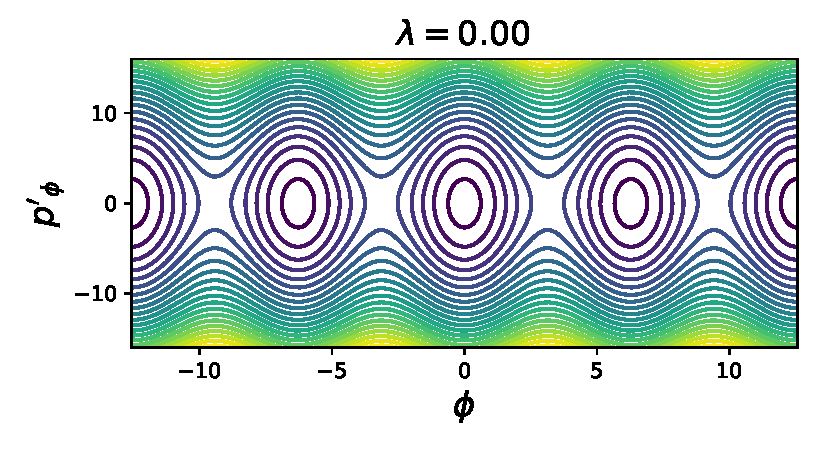
\includegraphics[width=0.49\textwidth]{{fig/lambd=0.00}.pdf}
    \includegraphics[width=0.49\textwidth]{{fig/lambd=0.15}.pdf}
    \includegraphics[width=0.49\textwidth]{{fig/lambd=0.30}.pdf}
    \includegraphics[width=0.49\textwidth]{{fig/lambd=0.45}.pdf}
    \includegraphics[width=0.49\textwidth]{{fig/lambd=0.60}.pdf}
    \includegraphics[width=0.49\textwidth]{{fig/lambd=0.75}.pdf}
    \includegraphics[width=0.49\textwidth]{{fig/lambd=0.90}.pdf}
    \includegraphics[width=0.49\textwidth]{{fig/lambd=1.05}.pdf}
    \caption{asdf}
\end{figure}

\subsection*{g)}
Firstly, we have
\begin{align*}
    p'_\phi = (mb^2 + I)\dot{\phi} \quad\quad \Rightarrow \quad\quad
    \dot{\phi} = \frac{1}{mb^2 + I}p'_\phi
\end{align*}
giving the Hamiltonian as a function of $\phi$ and $p'_\phi$ only:
\begin{align*}
    H &= \half \qty(m b^2\dot + I)\dot{\phi}^2 - mgb\cos{\phi} + I\alpha\phi \\
    &= \half \qty(m b^2\dot + I)\frac{1}{(mb^2 + I)^2}{p'_\phi}^2 - mgb\cos{\phi} + I\alpha\phi \\
    &= \half \frac{{p'_\phi}^2}{mb^2 + I} - mgb\cos{\phi} + mgb\lambda\phi \\
\end{align*}



\section*{Oppgave 2}
\subsection*{a)}


\subsection*{b)}
Conservation of energy gives that particle A and a must have a combined energy equal to that of particle B before the decacy.
\begin{align*}
    E_B &= E_A + E_a\\
    \sqrt{p_B^2c^2 + m_B^2c^4} &= \sqrt{p_A^2c^2 + m_A^2c^4} + \sqrt{p_a^2c^2 + m_a^2c^4}
\end{align*}
In the rest frame of A, $p_A = 0$, and conservation of momentum gives that $p_a^2 = p_B^2$ (total momentum before decay must equal total momentum after dacay). This gives

\begin{gather*}
    \sqrt{p_a^2 + m_B^2c^2} = \sqrt{m_A^2c^2} + \sqrt{p_a^2 + m_a^2c^2} \\
    \qty(\sqrt{p_a^2 + m_B^2c^2})^2 = \qty(\sqrt{m_A^2c^2} + \sqrt{p_a^2 + m_a^2c^2})^2 \\
    p_a^2 + m_B^2c^2 = m_A^2c^2 + p_a^2 + m_a^2c^2 + 2\sqrt{m_A^2c^2}\sqrt{p_a^2 + m_a^2c^2} \\
    \sqrt{p_a^2 + m_a^2c^2} = \frac{m_B^2c^2 - m_a^2c^2 - m_A^2c^2}{2m_Ac} \\
    p_a^2 + m_a^2c^2 = \frac{\qty(m_B^2c^2 - m_a^2c^2 - m_A^2c^2)^2}{4m_A^2c^2} \\
    p_a^2 + m_a^2c^2 = \frac{m_B^4c^4 + m_a^4c^4 + m_A^4c^4 - 2m_B^2m_a^2c^4 - 2m_B^2m_A^2c^4 + 2m_a^2m_A^2c^4}{4m_A^2c^2} \\
    p_a = \frac{\sqrt{m_B^4c^4 + m_a^4c^4 + m_A^4c^4 - 2m_B^2m_a^2c^4 - 2m_B^2m_A^2c^4 + 2m_a^2m_A^2c^4 - 4m_a^2m_A^2c^4}}{2m_Ac}
\end{gather*}
\begin{gather}\label{eqn:p_a}
    p_a = c\frac{\sqrt{m_B^4 + m_a^4 + m_A^4 - 2m_B^2m_a^2 - 2m_B^2m_A^2 - 2m_a^2m_A^2}}{2m_A}
\end{gather}


\subsection*{c)}
We have the invariant mass given as
\begin{gather*}
    m_{ab}^2c^2 = (p_a + p_b)^2 = (p_a + p_b)^\mu (p_a + p_b)_\mu
\end{gather*}

We write out the 4-vector with energy and regular momentum components
\begin{align*}
    (p_a + p_b)^\mu &= \qty(\frac{E_a + E_b}{c},\ \qty[\vec{p_a} + \vec{p_b}])\\
    (p_a + p_b)_\mu &= \qty(\frac{E_a + E_b}{c},\ -\qty[\vec{p_a} + \vec{p_b}])
\end{align*}
which gives the invariant mass
\begin{align*}
    m_{ab}^2c^2 = \frac{(E_a + E_b)^2}{c^2} - \qty[\vec{p_a} + \vec{p_b}]^2
\end{align*}
Inserting the relativistic energy (with $m_a = m_b = 0$)
\begin{align*}
    E_a &= \sqrt{p_a^2c^2 + m_a^2c^4} = p_ac \\
    E_b &= \sqrt{p_b^2c^2 + m_b^2c^4} = p_bc
\end{align*}
gives
\begin{align*}
    m_{ab}^2c^2 &= \frac{(p_ac + p_bc)^2}{c^2} - \qty[\vec{p_a} + \vec{p_b}]^2 \\
    &= p_a^2 + p_b^2 + 2p_ap_b - \vec{p_a}^2 - \vec{p_b}^2 - 2\vec{p_a}\cdot\vec{p_b}
\end{align*}
The squared vectors simply become their magnitudes squared ($\vec{p}^2 = p^2$), while the dot product can be written $\vec{p_a}\cdot\vec{p_b} = p_ap_b\cos{\theta_{ab}}$, where $\theta_{ab}$ is the angle between the vectors. This gives
\begin{align*}
    m_{ab}^2c^2 = 2p_ap_b - 2p_ap_b\cos{\theta_{ab}} = 2p_ap_b(1-\cos{\theta_{ab}})
\end{align*}
\begin{align}\label{eqn:m_ab}
    m_{ab}^2 = \frac{2}{c^2}p_ap_b(1-\cos{\theta_{ab}})
\end{align}

We observe that the decay $C \rightarrow bB$ from the refrence frame of $B$ is identical to the decay $B \rightarrow aA$ from the frence frame of $A$, solved in the last exercise. We therefore borrow equation (\ref{eqn:p_a}), substituting $(B, a, A)$ with $(C, b, B)$. Setting $m_b = 0$ gives
\begin{align}
    p_b = c\frac{\sqrt{m_C^4 + m_B^4 - 2m_C^2m_B^2}}{2m_B} = c\frac{\sqrt{(m_C^2 - m_B^2)^2}}{2m_B} = c\frac{m_C^2 - m_B^2}{2m_B}
\end{align}

We now need an expression for $p_a$.

Looking at the second decay from the refrence frame of $B$, we get the slightly different energy conservation, with $p_A^2 = p_a^2$ and $p_B = 0$. We also set $m_a = 0$.
\begin{gather*}
    E_B = E_A + E_a \\
    \sqrt{p_B^2c^2 + m_B^2c^4} = \sqrt{p_A^2c^2 + m_A^2c^4} + \sqrt{p_a^2c^2 + m_a^2c^4} \\
    \sqrt{p_B^2 + m_B^2c^2} = \sqrt{p_A^2 + m_A^2c^2} + \sqrt{p_a^2 + m_a^2c^2} \\
    m_Bc = \sqrt{p_a^2 + m_A^2c^2} + p_a \\
    (m_Bc - p_a)^2 = p_a^2 + m_A^2c^2 \\
    m_B^2c^2+ p_a^2 - 2m_Bp_ac = p_a^2 + m_A^2c^2
\end{gather*}
\begin{gather}
    p_a = c\frac{m_B^2 - m_A^2}{2m_B}
\end{gather}

Inserting this into equation (\ref{eqn:m_ab}) gives
\begin{align*}
    m_{ab}^2 = \frac{2}{c^2}c\frac{m_B^2 - m_A^2}{2m_B}c\frac{m_C^2 - m_B^2}{2m_B}(1-\cos{\theta_{ab}}) = \frac{(m_B^2 - m_A^2)(m_C^2 - m_B^2)}{2m_B^2}(1-\cos{\theta_{ab}})
\end{align*}


\end{document}
